\documentclass[11pt, oneside]{article}   	% use "amsart" instead of "article" for AMSLaTeX format
\usepackage{geometry}                		% See geometry.pdf to learn the layout options. There are lots.
\geometry{letterpaper}                   		% ... or a4paper or a5paper or ... 
%\geometry{landscape}                		% Activate for for rotated page geometry
%\usepackage[parfill]{parskip}    		% Activate to begin paragraphs with an empty line rather than an indent
\usepackage{graphicx}				% Use pdf, png, jpg, or eps§ with pdflatex; use eps in DVI mode
								% TeX will automatically convert eps --> pdf in pdflatex		
\usepackage{amssymb}
\usepackage{amsmath}

\DeclareMathOperator{\erf}{erf}
\DeclareMathOperator{\erfc}{erfc}
\DeclareMathOperator{\arccosh}{arccosh}
%\newcommand{\erf}{\operatorname{erf}}
%\newcommand{\erfc}{\operatorname{erfc}}

\title{Pulsed source modelling}
\author{}
%\date{}							% Activate to display a given date or no date

\begin{document}
\maketitle
%\section{}
%\subsection{}

Here, at the request of one of the reviewers we consider a hypothetical situation whereby the confined fields of cytokines arise not from the diffusion/consumption mechanism, but rather from short pulses of cytokine secretion by a cytokine producing cell. We show here that cytokine concentration profiles in such situation are not be consistent with our experimental data either 1) quantitatively, as their spatial extent would be much larger than that experimentally observed, or 2) qualitatively, as the shape of the fields would differ from the measured ones.

Thus we consider a problem of simple diffusion:
\begin{equation}
\frac{\partial c}{ \partial t} = D \nabla^2 c
\label{Eq: Diffusion3D}
\end{equation}
with the boundary condition of a given flux of cytokine molecules the cell wall (assuming a spherical cell of radius R):
\begin{eqnarray}
&4\pi R^2 D \frac{\partial c}{ \partial r} _{|r=R}= J(t),  \nonumber \\ 
& \frac{\partial c}{ \partial r} _{|r \rightarrow \infty} = 0,
\label{Eq: BoundCond_Diff3D}
\end{eqnarray}
where $J$ is the number of cytokine molecules produced by the cell per unit time.

While there is no time-dependent analytical solution to this problem, it can be readily solved numerically and, independently, some general qualitative considerations can be made. We will start with the general remarks and then show the numerical solutions for several conditions. For the numerical solutions we use standard partial differential equations (PDE) packages included with Matlab.

\emph{General remarks:} For the constant secretion rate $J$ the concentration profiles approach a steady state shape of $c = c_0/r$ with $c_0 = J/(4\pi D r)$. The approach is not uniform: the locations close to the cell reach steady state concentration roughly within time $\tau = R^2/D$ while those at distance $r$ arrive to the steady state after time $t \sim r^2/D$. Two observations follow from this: first, for the known parameters ($R\sim 5~\mu m$ and $D = 100~\mu m^2/s$) the concentration front propagation time is rather short: $\tau \sim 0.25~s$ and reaching the steady state at the distance of, say, 10 cell diameters from the source will take $\sim 100~s$. Second, the steady state concentration profile of $c = c_0/r$ is very different in shape from the experimentally measured dependence that is exponentially decaying with $r$. The $c = c_0/r$ dependence also extends much father from the cell than the exponentially decaying function.

When the formerly secreting cell stops producing cytokines, within time $\tau$ the concentration profile near the cell flattens out while the concentration field propagates outwards further increasing the field size while decreasing the cytokine concentration. Thus, at this stage the cytokine concentration profiles again are expected to have the shape very different from the exponentially decaying one, and the characteristic penetration length much larger than that experimentally observed.

The expected measurement from pulsing source in pure diffusion conditions then would be just averaging the above situations, and therefore would be inconsistent with our actual experimental results. The detailed numerical modelling presented below just confirms these general considerations.

\emph{Numerical modelling:} For modelling it is convenient to express distances in the units of $R$ and times in the units of $\tau$ (defined above) in the Eqs.~\ref{Eq: Diffusion3D}-\ref{Eq: BoundCond_Diff3D}. Then, introducing $t' = t/\tau$ and $\rho  = r/R$ we solve a rescaled diffusion equation:
\begin{equation}
\frac{\partial c}{ \partial t'} = \frac{1}{\rho^2}\frac{\partial}{\partial \rho} \left ( \rho^2 \frac{\partial c}{\partial \rho} \right )
\label{Eq: Diffusion3Drescaled}
\end{equation}
under appropriate boundary and initial conditions.

In addition to cytokine concentration fields we calculate a distance dependent cell response using $f(c) = \frac{1}{1+c*/c}$. In order to model the fact that cells do not respond to local cytokine concentrations immediately, but rather integrate cytokine signals for more than $\sim 10$~min (only IL-2 binding to its receptor lasts for $\sim 15$~min and there are further downstream reactions), we average cell response over $10$~min time.

We present here the examples of two general situations: 1) rare short pulses of cytokines, and 2) a cell switching from secreting to non-secreting state at the rate of few minutes. Other situations can be treated similarly.

\emph{Rare short pulses of cytokines:} 
As an illustrative example we consider here a cell that secretes cytokines for 5~min and then switches off for 55~min. For the average secretion rate of $\sim 10~$molecules per second, the cell has to produce 120 molecules per second during the secretion interval. 

\begin{figure}[h!]
	\centering
		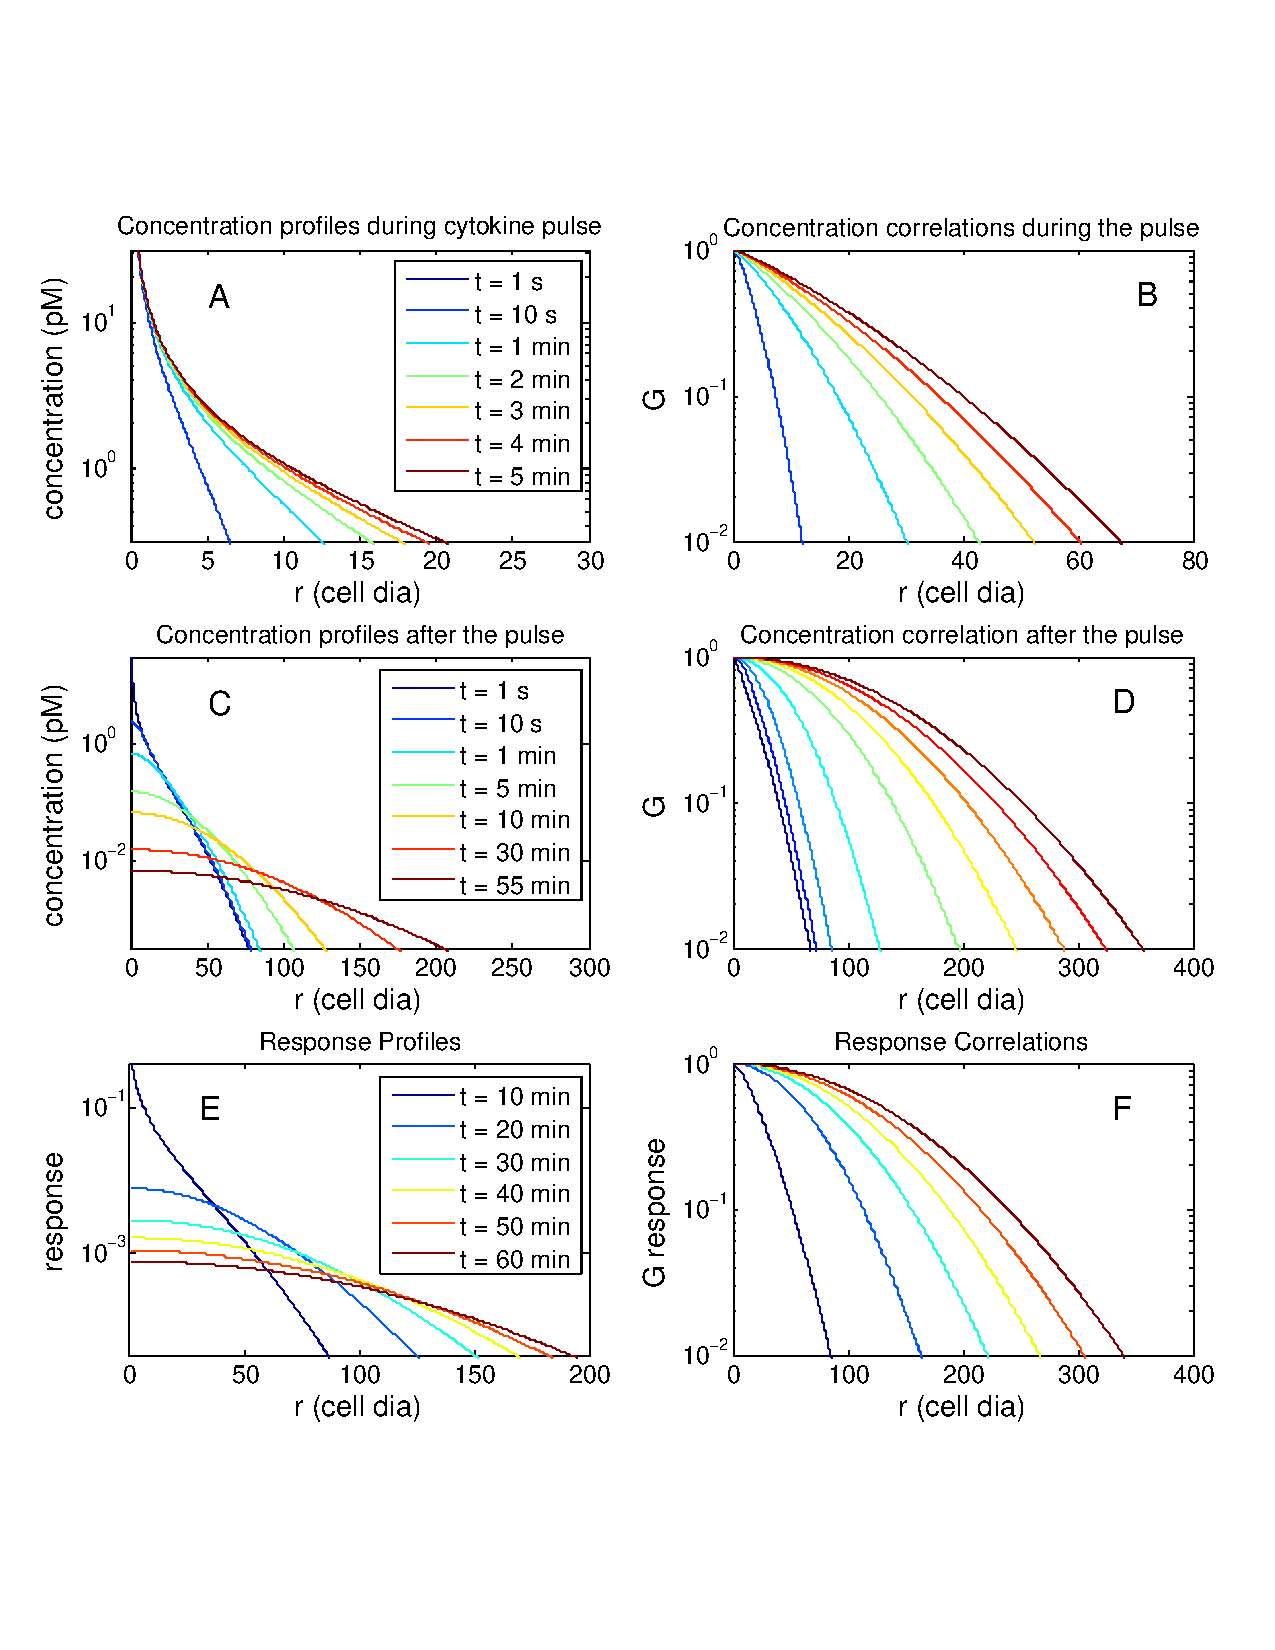
\includegraphics[width = 6 in]{TimeDependentProfilesPulse.pdf}
		\caption{\label{Fig:10min secr} The evolution of calculated concentration and response profiles, and their correlations during and after a 5 min pulse  of cytokines: (A) and (B) concentration profiles during the pulse and their correlations respectively, (C) and (D) concentration profiles and their correlations time $t$ after the termination of cytokine pulse, (E) and (F)}
\end{figure}

In Fig.~\ref{Fig:10min secr}, we present the changes in the expected concentration  profiles and their spatial correlation functions during secretion state and switched off state, and then the predicted response profiles and their spatial correlations. One can observe that the response curves have very different shapes from those experimentally observed: in semilogY scale the shape changes from convex during the secretion interval to concave when the source is switched off never approaching experimental curves that look almost linear in this scale. The corresponding correlation curves are always concave and thus different from linear in this scale  experimental curves. Both calculated response curves and their correlations extend much further from the source than experimentally measured.

\emph{Pulsing source of cytokines:} 
Here we consider a cell that switches secretion on and off periodically with 10 min period (5 min on and 5 min off).  Again for the average secretion rate of $\sim 10~$molecules per second, the cell has to produce now 20 molecules per second during the secretion interval. We present the results of the first 6 cycles in Fig.~\ref{Fig:periodic source}.

\begin{figure}[h!]
	\centering
		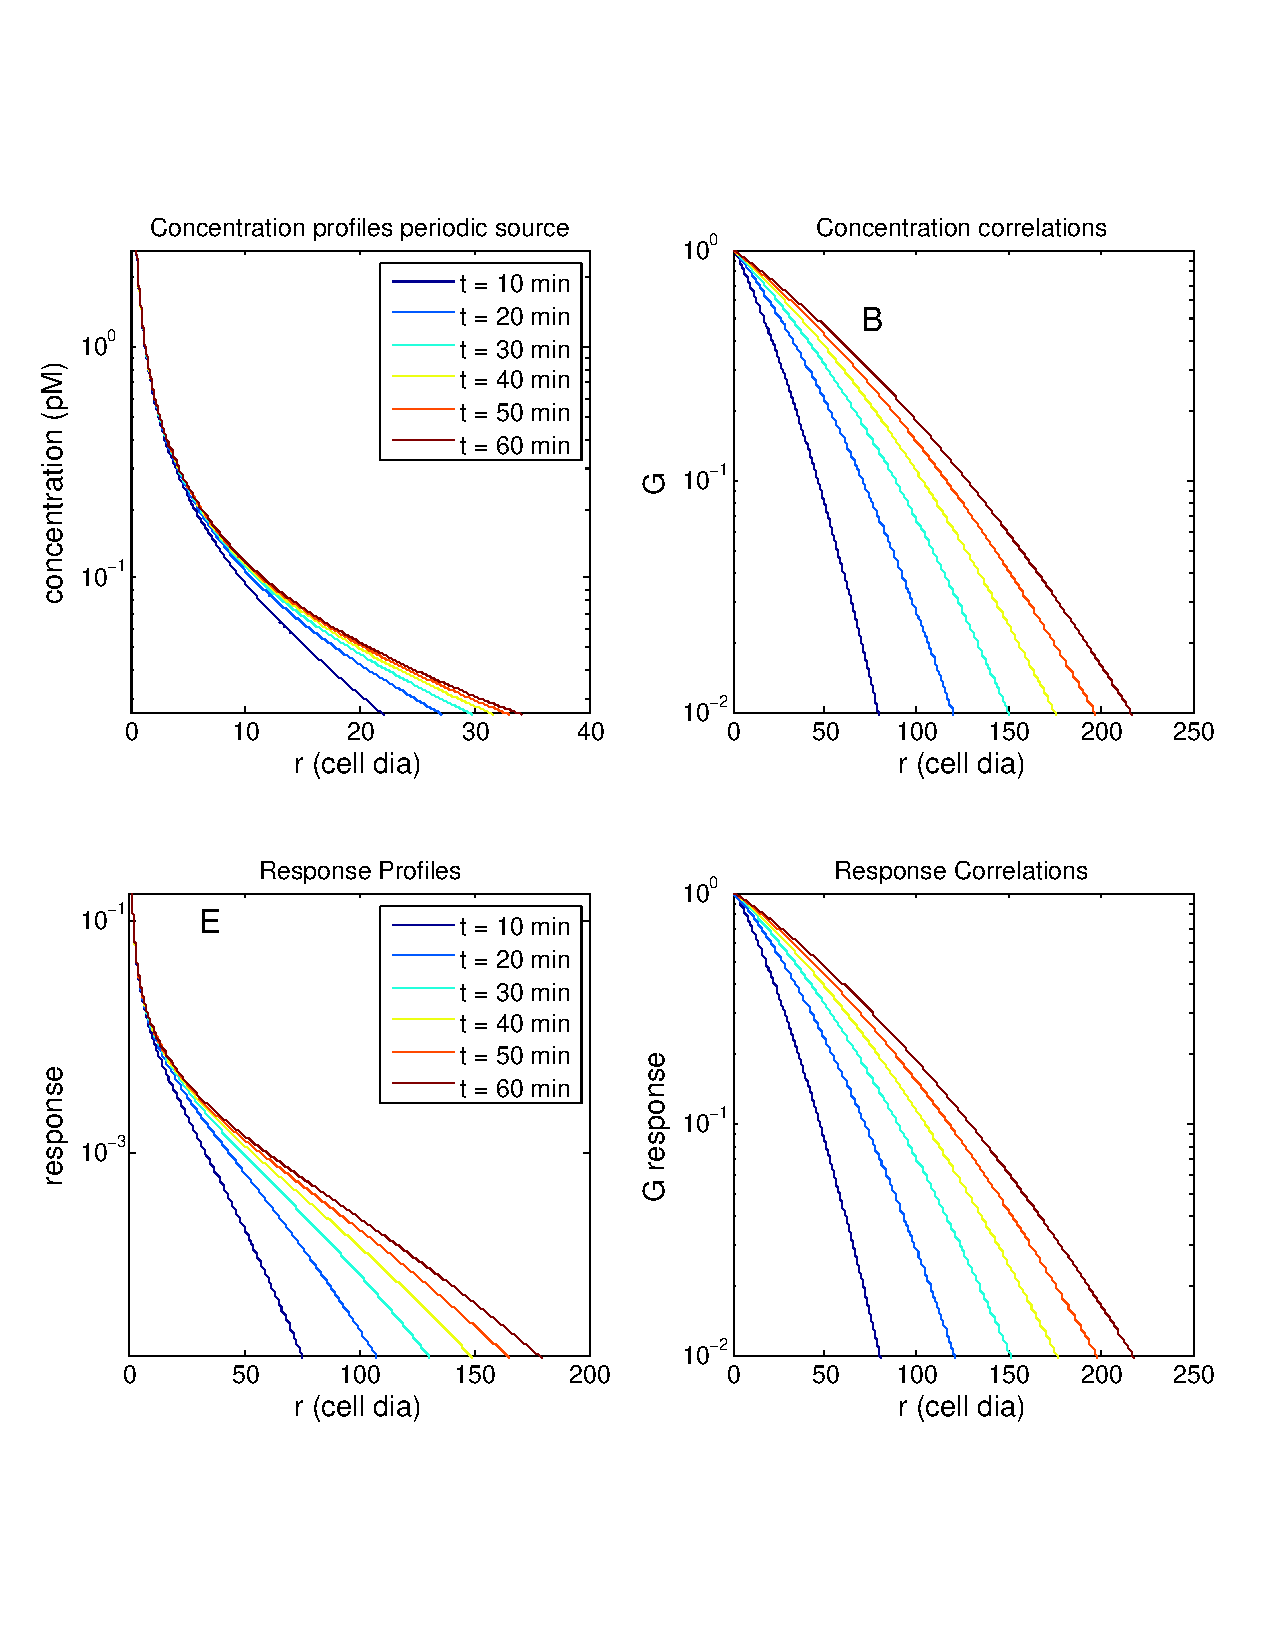
\includegraphics[width = 6 in]{TimeDependentProfilesPeriodic.pdf}
		\caption{\label{Fig:periodic source} The evolution of calculated concentration and response profiles, and their correlations during and after a 5 min pulse  of cytokines: (A) and (B) concentration profiles during the pulse and their correlations respectively, (C) and (D) concentration profiles and their correlations time $t$ after the termination of cytokine pulse, (E) and (F)}
\end{figure}

As in the previous case, all of the calculated curves and their correlations have shapes very different from simple singe-exponential behavior. They also extend much further from the source than the dependencies measured in experiments.

Thus this numerical modelling confirms our conclusion that the measured distance dependences of responses to IL-2 result from diffusion/consumption kinetics and not from the diffusion kinetics alone. Other strong evidences for that are: 1) persistence of cytiokine secretion (thus no really pulsing sources of cytokines), 2) quantitative consistency of our measurements with diffusion/consumption model, and, finally, 3) the very presence of cytokine consumption by the cells that cannot be dismissed.

\end{document}  